\documentclass[
hyperref={colorlinks,citecolor=blue,linkcolor=blue,urlcolor=blue}
]{beamer}
\usetheme{metropolis}           % Use metropolis theme
\useoutertheme{metropolis}
\useinnertheme{metropolis}

\usepackage{tikz}
\usetikzlibrary{patterns, backgrounds}
\usepackage{pgfplots}
\usepgfplotslibrary{groupplots, fillbetween}

\usepackage{xcolor}
% Using the Set1 palette from colorbrewer (http://colorbrewer2.org/#type=qualitative&scheme=Set1&n=3)
\definecolor{myred}{HTML}{e41a1c}
\definecolor{myblue}{HTML}{377eb8}
\definecolor{mygreen}{HTML}{4daf4a}
\definecolor{mygray}{gray}{0.6}

\title{Some TikZ and PGFplot examples}
\subtitle{(Tailored toward environmental economics topics)}
\author{Grant R. McDermott}
\date{\href{mailto:grantmcd@uoregon.edu}{grantmcd@uoregon.edu}}
\institute{University of Oregon}
\begin{document}
	\maketitle

%\section*{Equimarginal principle}

%----------- new slide ---------------------------------------%

\begin{frame}{Equimarginal principle}

	\begin{figure}[!h]
		\centering
		\begin{tikzpicture}
		\begin{groupplot}[
		axis lines=middle,
		xlabel=Abatement,
		ylabel near ticks, 
%		every axis x label/.style={
%			at={(ticklabel* cs:1.01)},
%			anchor=west,
%		},
		xlabel style={at={(ticklabel* cs:1.05)}, anchor=north},
		every axis y label/.style={
			at={(ticklabel* cs:1)},
			anchor=south,
		},
		group style={
			group name = equimarginal,
			group size = 1 by 2,
			xlabels at = edge bottom,
			xticklabels at = edge bottom,
			vertical sep = 0.75cm
		},
		%			footnotesize,
		width = 0.9\textwidth, %% As big as this example can be without spilling over onto the next slide
		height = 0.5\textheight, %% ditto
		%			ticks = none,
		ytick=\empty,
		xtick={2}, xticklabels={{\color{myred}$A^*$}},
		xmin = 0, 
		xmax = 5, 
		]
		\nextgroupplot[ymax=22, ylabel=\$, xlabel=Abatement]
		\addplot[name path=TB, domain={0:4.5}, thick] {8*x-x^2} node[right]{$TB$};
		\addplot[name path=TC, domain={0:4.5}, thick] {x^2} node[right]{$TC$};
		%% Show maximum difference
		\draw[decoration={brace,mirror,raise=3pt},decorate,myred]
		(200, 47) -- node[right=4pt] {\footnotesize\color{myred}max} (200,116);
		%% Top part of vertical line
		\coordinate (top) at (axis cs:2,\pgfkeysvalueof{/pgfplots/ymax});
		\nextgroupplot[ymax=12, ylabel=\$/unit]
		\addplot[name path=MB, domain={0:4}, thick] {8-2*x} node[above right]{$MB$};
		\addplot[name path=MC, domain={0:4}, thick] {2*x} node[right]{$MC$};
		%% Bottom part of vertical line
		\coordinate (bottom) at (axis cs:2,\pgfkeysvalueof{/pgfplots/ymin});
		\end{groupplot}
		\draw [densely dashed, myred] (top) -- (bottom);
		\end{tikzpicture}
	\end{figure}

\end{frame}

%----------- new slide ---------------------------------------%
%
%\begin{frame}{Externality with deadweight loss}
%	
%	\begin{figure}
%		\centering
%		\begin{tikzpicture}[%yscale=1.05, 
%		xscale=1]
%		\begin{axis}[
%		width = .9\textwidth,
%		height = .9\textheight,
%		axis lines=middle,
%		xlabel=Emissions ($e$),
%		ylabel=Price (\$),
%		ylabel near ticks,  
%		every axis x label/.style={
%			at={(ticklabel* cs:1.05)},
%			anchor=west,
%		},
%		xlabel style={at={(ticklabel* cs:1)}, anchor=north},
%		every axis y label/.style={
%			at={(ticklabel* cs:1.05)},
%			anchor=south,
%		}, 
%		xtick={3,5}, xticklabels={$e^*$,$e_m$},
%		ytick={5, 21}, yticklabels={$p_m$,$p^*$},
%		xmin = 0, 
%		xmax = 8, 
%		ymin = 0, 
%		ymax = 60
%		]
%		
%		%% MB curve
%		\addplot[name path=MB, domain={0:5.5}, thick] {30-x^2} node[above right]{$MB$};
%		%%% PMC curve
%		\addplot[name path=PMC, domain={0:7}, thick] {5} node[right]{$PMC$};
%		%%% Define MEC curve
%		\addplot[name path=MEC, domain={0:6}, thick, dashed] {\x^2+7} node[below right]{$MEC$};
%		%% SMC curve
%		\addplot[name path=SMC, domain={0:6}, thick] {x^2+12} node[above right]{$SMC$};
%		
%		%% Equilibria
%		\coordinate (yend) at (0,50);
%		\coordinate (xend) at (7,0);
%		\path [name intersections={of=MB and PMC, by={eqm_m}}]; 
%		\path [name intersections={of=MB and SMC, by={eqm_s}}]; 
%		\draw[densely dashed]  (yend |- eqm_m) -- (eqm_m) -- (eqm_m |- xend);
%		\draw[densely dashed]  (yend |- eqm_s) -- (eqm_s) -- (eqm_s |- xend);
%		
%		%% DWL
%		\addplot[fill=myred!50]fill between[of=SMC and MB, soft clip={domain=3:5}];
%		\node[coordinate, pin={[pin edge={myred, thick}]30:{\textbf{{\color{myred}DWL}}}}, thick] at (axis cs:4.8,20){};
%		
%		\end{axis}
%		\end{tikzpicture}
%	\end{figure}
%\end{frame}

%----------- new slide ---------------------------------------%

\begin{frame}{Externality with deadweight loss}

\begin{figure}
	\centering
	\begin{tikzpicture}[%yscale=1.05, 
	xscale=1]
	\begin{axis}[
	width = .9\textwidth,
	height = .9\textheight,
	axis lines=middle,
	xlabel=Emissions ($e$),
	ylabel=Price,
	ylabel near ticks,  
	xlabel style={at={(ticklabel* cs:1)}, anchor=north},
	ylabel style={at={(ticklabel* cs:1)}, anchor=south},
%	every axis y label/.style={
%		at={(ticklabel* cs:1.05)},
%		anchor=south,
%	}, 
	xtick={3, 5}, xticklabels={$e^*$,$e_m$},
	ytick={15, 31}, yticklabels={$p_m$,$p^*$},
	xmin = 0, 
	xmax = 8, 
	ymin = 0, 
	ymax = 75
	]
	
	%% MB curve
	\addplot[name path=MB, domain={0:7}, thick] {40-x^2} node[pos=0, above right]{$MB$};
	%%% PMC curve
	\addplot[name path=PMC, domain={0:7}, thick] {15} node[right]{$PMC$};
	%%% Define MEC curve
	\addplot[name path=MEC, domain={0:6.5}, thick, dashed] {\x^2+7} node[right]{$MEC$};
	%% SMC curve
	\addplot[name path=SMC, domain={0:6.5}, thick] {x^2+22} node[above right]{$SMC$};
	
	%% Equilibria
	\coordinate (yend) at (0,75);
	\coordinate (xend) at (8,0);
	\path [name intersections={of=MB and PMC, by={eqm_m}}]; 
	\path [name intersections={of=MB and SMC, by={eqm_s}}]; 
	\draw[densely dashed]  (yend |- eqm_m) -- (eqm_m) -- (eqm_m |- xend);
	\draw[densely dashed]  (yend |- eqm_s) -- (eqm_s) -- (eqm_s |- xend);
	
	%% DWL
	\addplot[fill=myred!50]fill between[of=SMC and MB, soft clip={domain=3:5}];
	\node[coordinate, pin={[pin edge={myred, thick}]25:{\textbf{{\color{myred}DWL}}}}, thick] at (axis cs:4.75,25){};
	
	\end{axis}
	\end{tikzpicture}
\end{figure}
\end{frame}

%----------- new slide ---------------------------------------%

\begin{frame}{Tradeable permits}

	\begin{figure}
		\centering
		\begin{tikzpicture}%[scale=1.25]
		
		%% First y-axis (and shared x-axis)
		\begin{axis}[
		width = .85\textwidth,
		height = .9\textheight,
		axis x line*=bottom,
		axis y line=left,
		xmin=0, xmax=20,
		ymin=0, ymax=35,
		xtick=\empty,
		ytick=\empty,
		xtick={10,14}, xticklabels={{\color{myred}10} {\color{myblue}(10)},{\color{myred}14} {\color{myblue}(6)}},
		ytick={7,9}, yticklabels={{\color{gray} 7}, 9},
		xlabel=$\longleftarrow$ Abatement (20 tonnes total) $\longrightarrow$,
		ylabel={\color{myred} \$/unit},
		ylabel style={at={(ticklabel* cs:1.05)}, anchor=south east},
		]
		% MAC_1 curve
		\addplot[name path=MAC1, domain={0:20}, thick, myred] {(2+1/2*x)} node[above left]{$MAC_1$};
		
		% MAC_2 curve
		\addplot[name path=MAC2, domain={0:20}, thick, myblue] {30-1.5*x} node[pos=0,anchor=south west]{$MAC_2$};
		
		% Equilibria
		%% Have to multiply all these numbers by 10. (Why? Not sure...)
		\coordinate (xorig) at (0,0);
		\coordinate (xend) at (200,0);
		\coordinate (yend1) at (0,350); 
		\coordinate (yend2) at (200,350);
		
		\path [name intersections={of=MAC1 and MAC2, by={eqm_trade}}];
		\draw[densely dashed]  (eqm_trade) -- (eqm_trade |- xorig);
		\draw[densely dashed]  (xorig |- eqm_trade) -- (eqm_trade -| xend);
		
		% Uniform allotment
		\addplot[name path=u, draw=none] (10,0) -- (100,350);
		\path [name intersections={of=MAC1 and u, by={eqm_u1}}];
		\path [name intersections={of=MAC2 and u, by={eqm_u2}}];
		
		\draw[densely dashed, gray]  (xorig |- eqm_u1) -- (eqm_u1);
		\draw[densely dashed, gray]  (eqm_u2) -- (xend |- eqm_u2);
		\draw[densely dashed, gray]  (eqm_u2) -- (eqm_u2 |- xorig);
		
		%% Gains from trade
		\addplot[name path=g, draw=none, domain={0:20}] {(9)};
		\addplot[fill=myred!50]fill between[of=g and MAC1, soft clip={domain=10:14}];
		\addplot[fill=myblue!50]fill between[of=MAC2 and g, soft clip={domain=10:14}];
		%	\node[coordinate, pin={[pin edge={myred, thick}]30:{\textbf{{\color{myred}DWL}}}}, thick] at (axis cs:4.8,20){};
		
		\end{axis}
		
		%% Second y-axis
		\begin{axis}[
		width = .85\textwidth,
		height = .9\textheight,
		axis y line=right,
		axis x line=none,
		xmin=0, xmax=20,
		ymin=0, ymax=35,
		ylabel={\color{myblue} \$/unit},
		ylabel style={at={(ticklabel* cs:1.05)}, anchor=north east},
		ytick=\empty,
		ytick={15,9}, yticklabels={{\color{gray} 15}, 9},
		]
		\end{axis}
		
		\end{tikzpicture}
	\end{figure}
\end{frame}

%----------- new slide ---------------------------------------%

\begin{frame}{Public goods taxonomy}
	\begin{figure}
		\centering
		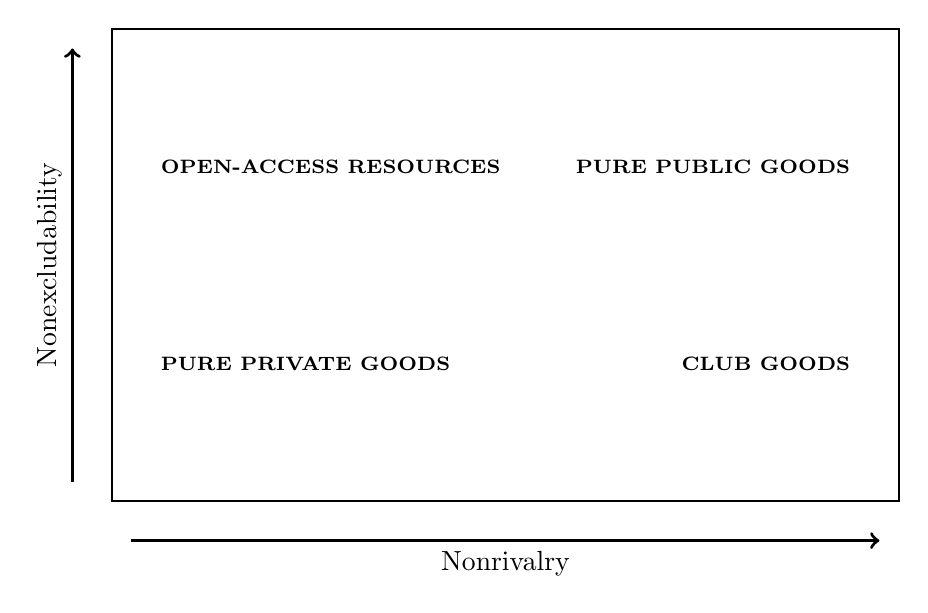
\begin{tikzpicture}%[scale=.8]
		\draw [<->,thick] (0,-0) rectangle (10,6);
		\draw [->, very thick] (0.25,-0.5) -- (9.75,-0.5) node [pos=0.5, below] {Nonrivalry}; 
		\draw [->, very thick] (-0.5,0.25) -- (-0.5,5.75) node [rotate=90, pos=0.5, above] {Nonexcludability};
		\node[right] at (0.5,1.75) {\scriptsize \textbf{PURE PRIVATE GOODS}};
		\node[right] at (0.5,4.25) {\scriptsize \textbf{OPEN-ACCESS RESOURCES}};
		\node[left] at (9.5,1.75) {\scriptsize \textbf{CLUB GOODS}};
		\node[left] at (9.5,4.25) {\scriptsize \textbf{PURE PUBLIC GOODS}};
		\end{tikzpicture}
	\end{figure}
\end{frame}


\begin{frame}{Environmental Kuznets curve}
	\begin{figure}
		\centering
		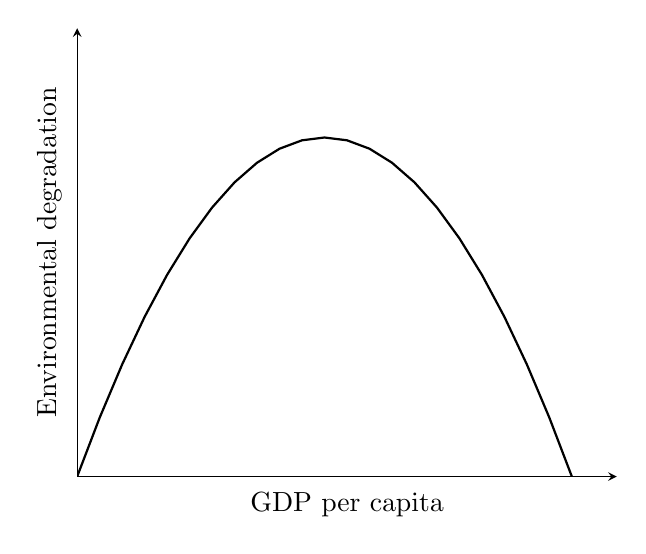
\begin{tikzpicture}
		\begin{axis}[
		axis lines=middle,
		xlabel=GDP per capita,
		ylabel=Environmental degradation,
		xlabel near ticks, 
		ylabel near ticks, 
		xmax=12,xmin=0,
		ymin=0,ymax=40,
		ytick=\empty, 
		xtick=\empty
		]
		%		\addplot[name path=EKC, domain={0:12}, thick] {(x+9)-(x-3)^2+10};
		\addplot[name path=EKC, domain={0:12}, thick] {11*x-x^2};
		\end{axis}
		\end{tikzpicture}
	\end{figure}
\end{frame}

\end{document}